% vim:autoindent:set textwidth=78:
\chapter{Working with Projections}\label{chp:projections}\index{Projections!working with}
QGIS supports on-the-fly projection of vector layers. This feature allows you
to display layers with different coordinate systems and have them overlay
properly. 
\section{Overview of Projection Support}
QGIS has support for approximately 2,700 known projections. 
Projections are stored in a Sqlite database that is installed with QGIS.
%Appendix \ref{app:datamodel}  contains information about the database and the schema. 
Normally you do not need to manipulate the database directly. In fact,
doing so may cause projection support to fail. Custom projections are
stored in a user database. See Section \ref{sec:customprojections} for
information on managing your custom projections.

The projections available in QGIS are based on those defined by
EPSG\index{EPSG} and are
largely abstracted from the spatial\_references table in
PostGIS\index{PostGIS} version 1.x.
Note that the identifiers used in QGIS do not correspond to the EPSG or
PostGIS spatial reference identifiers. The EPSG and PostGIS identifiers are
present in the database and can be used to specify a projection in QGIS.

In order to use OTF projection, your data must contain information about its
coordinate system. For PostGIS layers QGIS uses the spatial reference
identifier that was specified when the layer was created. For data supported
by OGR, QGIS relies on the presence of a format specific means of specifying
the coordinate system. In the case of shapefiles, this means a file containing
the Well Known Text (WKT)\index{WKT} specification of the the coordinate system. The
projection file has the same base name as the shapefile and a prj extension.
For example, a shapefile named lakes.shp would have a corresponding projection
file named lakes.prj.


%\section{Requirements}
%QGIS uses the Proj4 to provide projection support. 
\section{Getting Started}
At startup, QGIS does not have On-the-Fly (OTF) projection enabled. To use OTF
projection, you must open the \textit{Project Properties} dialog, select a
projection for the map,  and enable projections.  There are two ways to open
the \textit{Project Properties} dialog:
\begin{compactenum}
\item Select \textit{Project Properties} from the \textit{Settings} menu
\item Click on the projector icon in the lower right-hand corner of the
statusbar
\end{compactenum}
\begin{Tip}
 \caption{\textsc{Project Properties Dialog}}
\qgistip{
If you open the \textit{Project Properties} dialog from the Settings menu, you must
click on the \textit{Projection} tab to view the projection settings. Opening
the dialog from the projector icon will automatically bring the
\textit{Projection} tab to the front.
}
\end{Tip}
The Projection dialog contains four important components as numbered in Figure
\ref{fig:projections} and described below.
\begin{figure}[h]
   \begin{center}
   \caption{Projection Dialog (OS X)}\label{fig:projections}\smallskip
   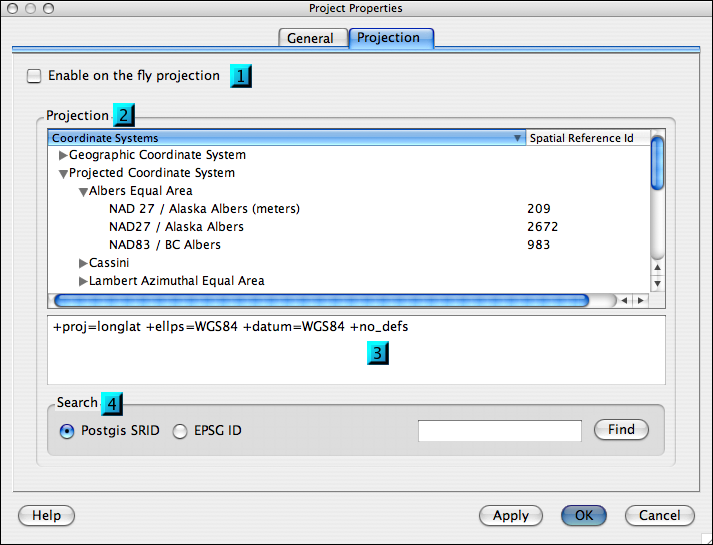
\includegraphics[scale=.70]{qgis_user_guide_images/projectiondialog}
\end{center}  
\end{figure}
\begin{compactenum}
\item Enable projections\index{Projections!enabling} - this checkbox is used to enable or disable OTF
projection. When off, no projection takes place and each layer
is drawn using the coordinates as read from the data source. When on, the
coordinates in each layer are projected to the coordinate system of the map
canvas.
\item Projections - this is a list of all projection supported by QGIS,
including Geographic, Projected, and Custom coordinate systems. To use a
coordinate system, select it from the list by expanding the appropriate node
and selecting the projection.
\item Proj4 text - this is the projection string used by the Proj4 projection
engine. This text is read-only and provided for informational purposes.
\item Search - if you know the PostGIS or EPSG identifier for a projection,
you can use the search feature to find it. Enter the identifier and click on
\textit{Find}.

\end{compactenum}
\subsection{Specifying a Projection}\index{Projections!specifying}
QGIS automatically sets the map projection to the coordinate system of the first
layer loaded. One way to specify the map projection is to first load a layer
with the projection you want for the entire map. Then open the \textit{Project Properties} 
dialog and click on the \textit{Enable on the fly projection} checkbox. You
can now close the \textit{Project Properties} dialog and add additional layers
to the map. 

If you have already added layers and want to enable OTF projection, open the 
\textit{Project Properties} dialog and find the projection or geographic
coordinate system you want to use in the list of projections. Alternatively
you can use the search feature as described in the previous section.

\section{Custom
Projections}\label{sec:customprojections}\index{Projections!custom}
If QGIS doesn't have the projection you need, you can define a custom
projection. To define a projection, select \textit{Custom Projections} from
the \textit{Settings} menu. Custom projections are stored in your QGIS user
database. In addition to your projections, this database contains your spatial
bookmarks and other custom data. 

At version 0.7 of QGIS, defining a custom projection requires a good
understanding of the Proj.4 projection library. To begin, refer to
Cartographic Projection Procedures for the UNIX Environment�A User�s Manual by 
Gerald I. Evenden, U.S. Geological Survey Open-File Report 90-284, 1990
(available at \url{ftp://ftp.remotesensing.org/proj/new\_docs/OF90-284.pdf}). This
manual describes the use of the \textit{proj} and related command line
utilities. The cartographic parameters used with \textit{proj} and described in
the user manual are the same as those used by QGIS. 

The Custom Projections dialog requires only two parameters to define a user
projection: 1) a descriptive name, and 2) the cartographic parameters. To
create a new projection, click the \textit{New} button and enter a descriptive
name and the projection parameters. Figure
\ref{fig:customprojections} shows the dialog with an example projection. The
parameters shown were entered based on a knowledge of the projection and the
information found in OF90-284.

\begin{figure}[h]
   \begin{center}
   \caption{Custom Projection Dialog (OS X)}\label{fig:customprojections}\smallskip
   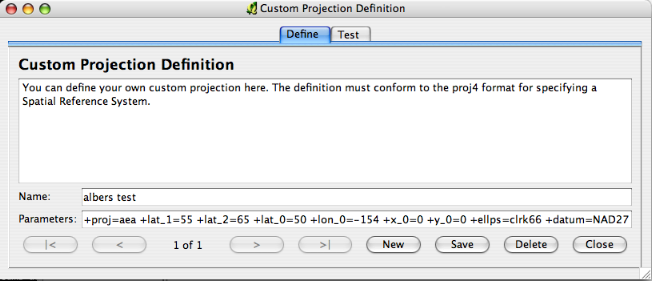
\includegraphics[scale=.70]{qgis_user_guide_images/customprojection}
\end{center}  
\end{figure}

You can test your projection parameters to see if they give sane results by
clicking on the \textit{Test} tab and pasting your projection parameters into
the \textit{Parameters} field. Then enter known WGS 84 latitude and longitude
values in North and East fields respectively. Click on \textit{Calculate} and
compare the results with the known values in your projected coordinate system. 
